\documentclass[a4paper, 12pt, colorlinks=true, linkcolor=black, urlcolor=blue, citecolor=blue, hidelinks]{article}
\usepackage{xcolor}

\usepackage[a-1b]{pdfx}

\usepackage[italian]{babel} % Language
%Font
\usepackage{fontspec}
\usepackage{comment}
\usepackage{listings}
\usepackage{xcolor}

\begin{comment}
    add a specific font here
    \setmainfont{MiloTE}[
      Path = ./Resources/Font/,
      Extension = .ttf,
      BoldFont = MiloTE-Bold,
      ItalicFont = MiloTE-Ita,
    ]
\end{comment}

\usepackage{graphicx}
\usepackage{geometry}
\usepackage{csquotes}
\geometry{a4paper,inner=4cm,outer=3cm,top=3cm,bottom=2.5cm}

\usepackage{float} % Required for the [H] option
\usepackage{caption}
%\captionsetup[figure]{font=small,labelfont=small}

\usepackage{setspace}
\setstretch{1.5}
\setlength{\parindent}{20pt}
%Bibliografia
\usepackage[backend=biber, style=numeric, sorting=none]{biblatex}


\usepackage{fontspec}
\begin{document}
\pagenumbering{roman}

\begin{titlepage} 
      \begin{center}
            \thispagestyle{empty}
            \begin{spacing}{2.0}
                \Large{\textbf{University of Pauda}
            \end{spacing}
            
\includegraphics[width=8.0cm]{Resources/UNIPD_Logo.png}
            \begin{spacing}{2.0}
                \large{\textbf{AIoT Basics using Containerization}}
            \end{spacing}
            \begin{spacing}{1.0}
                \Large{{Exercises}}\\
            \end{spacing}
            \vfill
            \begin{spacing}{1.0}
            \vspace{1.0cm}
            \raggedleft{\large{Student: \textit{\textbf{Lorenzo Albertin}}}}\\
            \raggedleft{\large{Student ID: \textit{\textbf{220160}}}}
            \end{spacing}
            \vspace{2.0cm}
                \large{ACCADEMIC YEAR 2025-2026}
            
        \end{center}
    \end{titlepage}
\tableofcontents % Table of contents
\newpage

\pagenumbering{arabic}
\setlength{\parindent}{0pt}
\setcounter{page}{1}
\section{Exercise 1 - EdgeImpulse} %Introduction
To complete the first exercise, I decided to classify the same items used in the provided demo.
In particular, I took 20 pictures of a coin, 20 pictures of a pen and 20 pictures of the background.\bigskip

After the training with an 80/20 split, I obtained the following results:

\begin{figure}[h!]
    \centering
    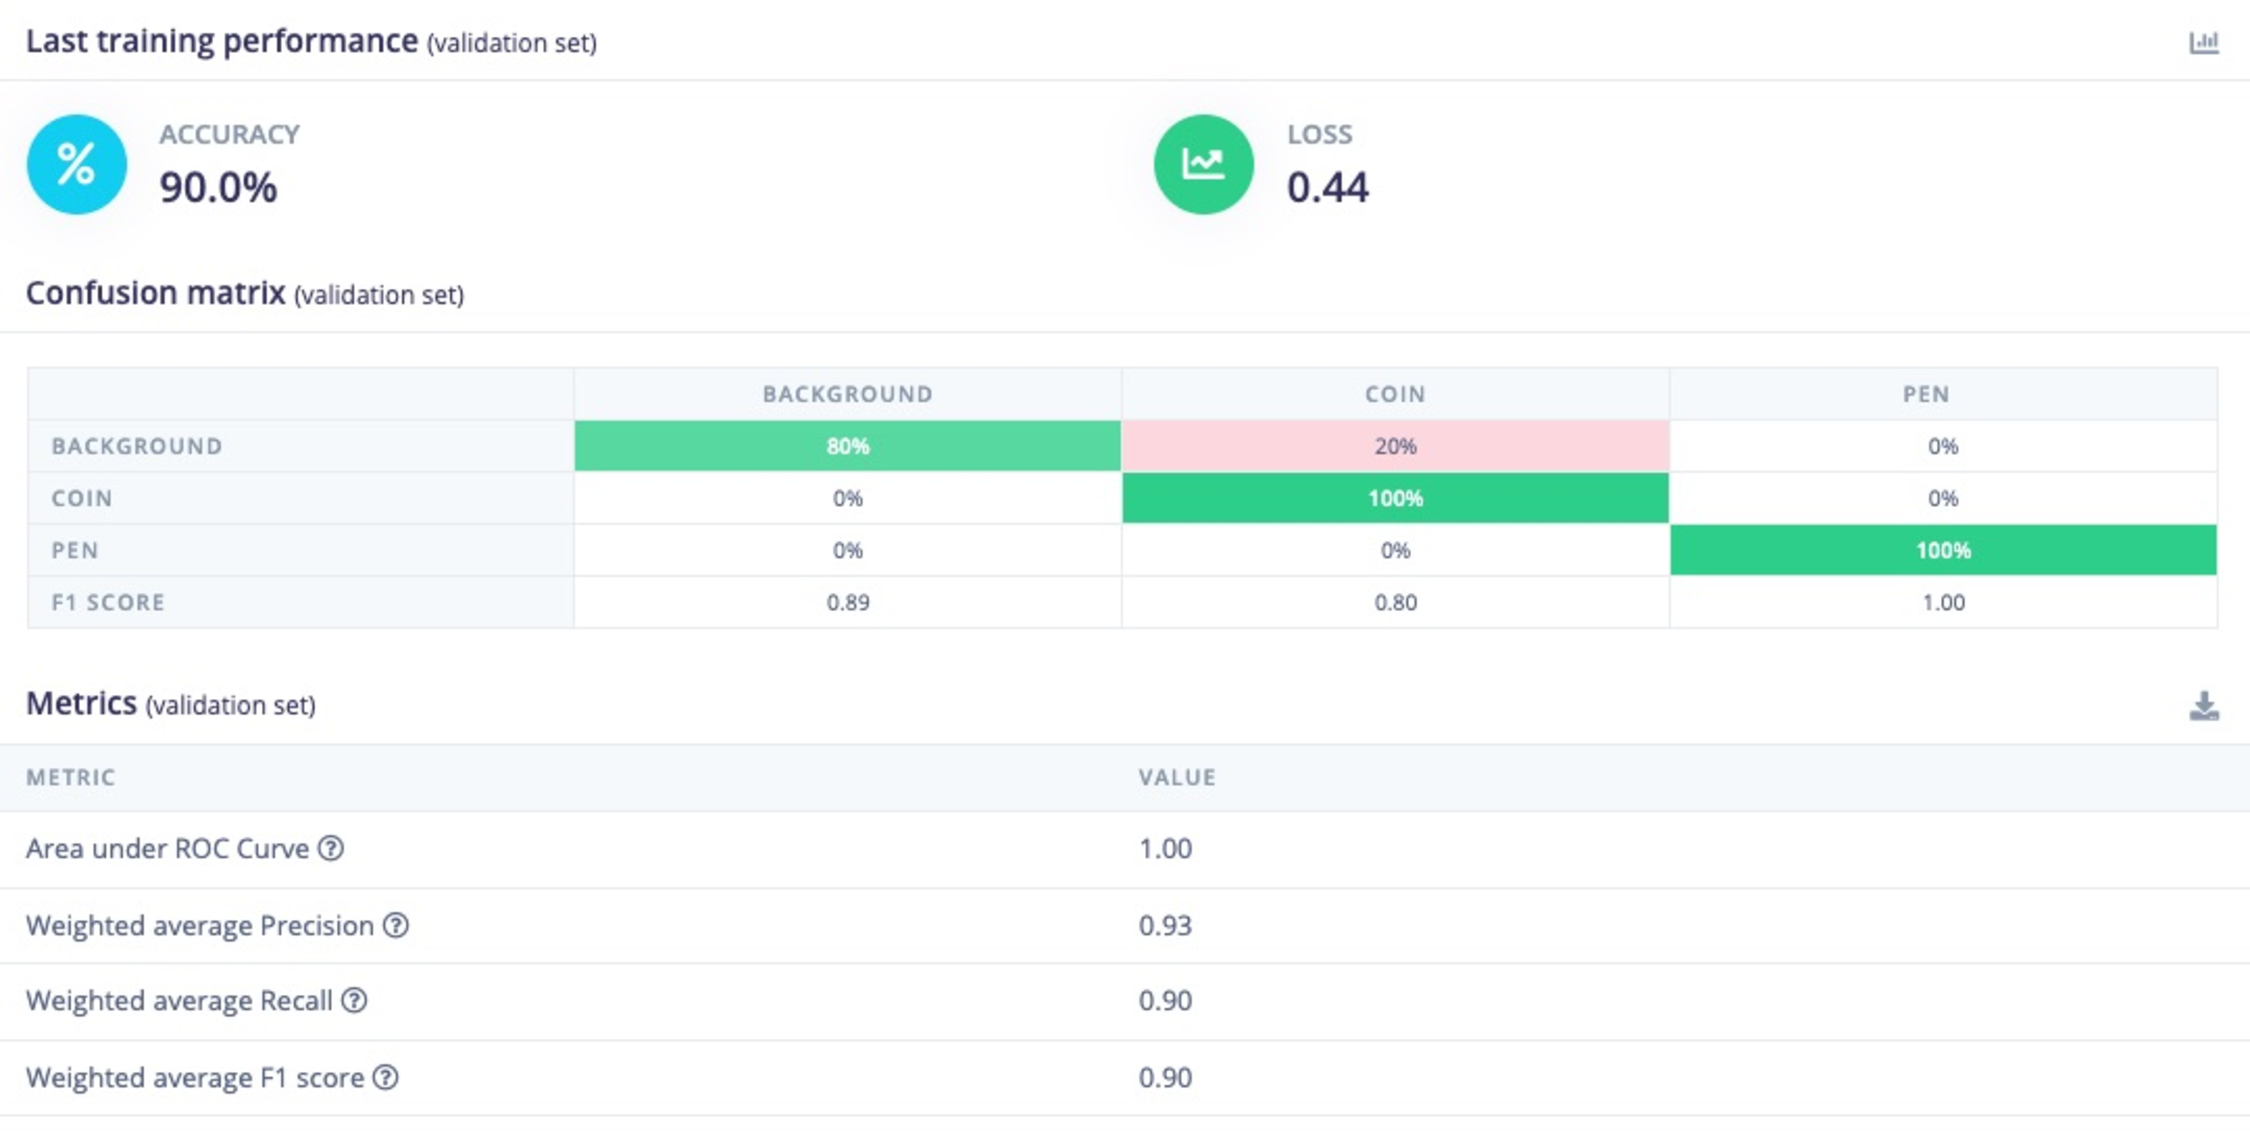
\includegraphics[width=0.8\linewidth]{Resources/Training_results.pdf} % <-- replace with your filename
    \caption{Training results}
\end{figure}

I also tested the model on the validation set, achieving an accuracy of 100\% as shown in the following screenshot:

\begin{figure}[h!]
    \centering
    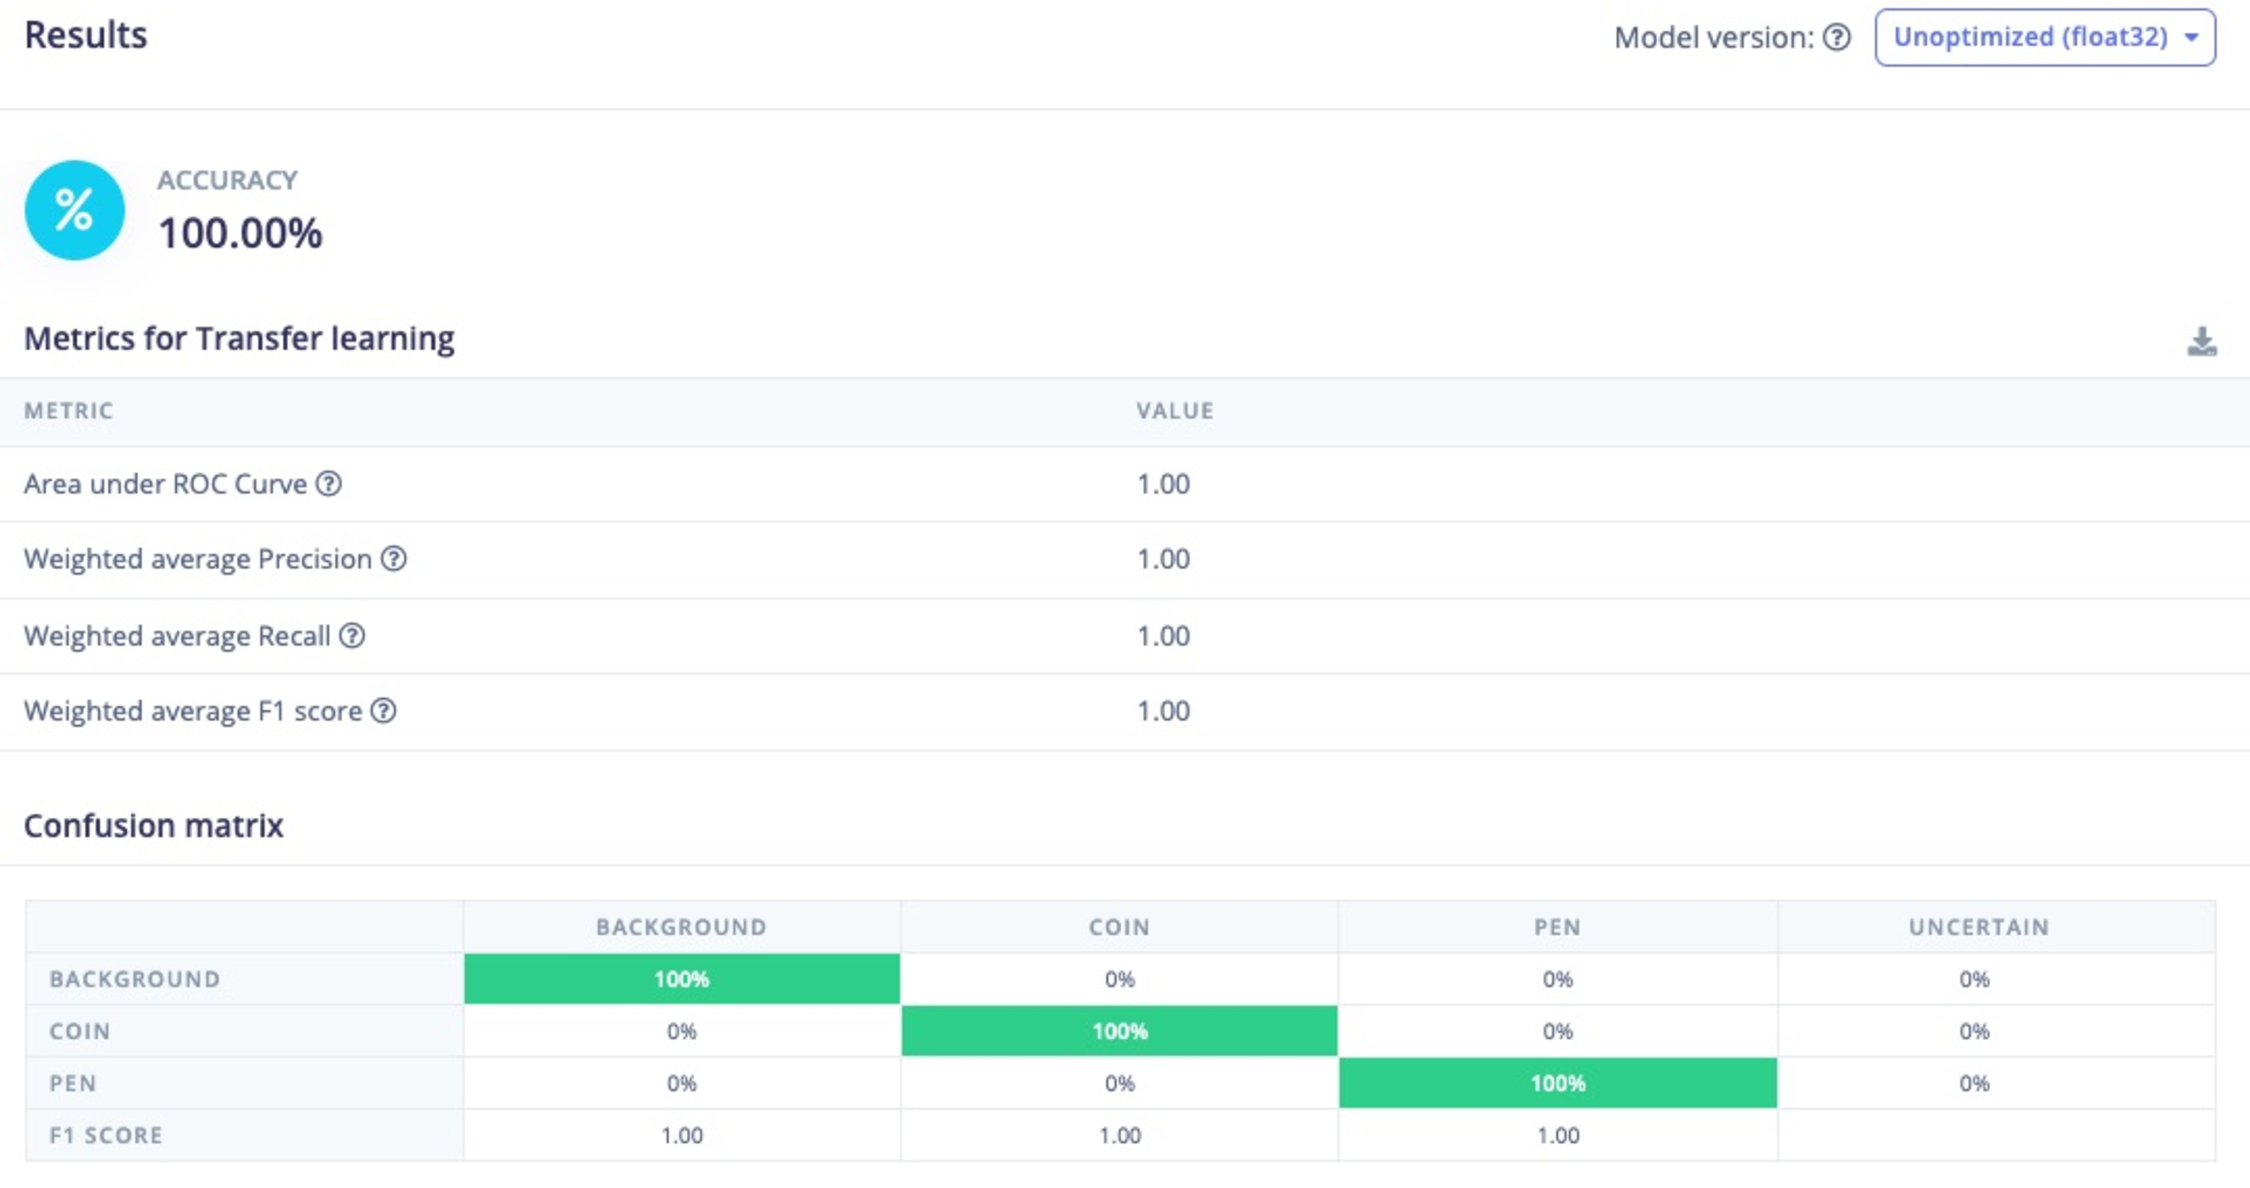
\includegraphics[width=0.8\linewidth]{Resources/Validation_results.pdf} % <-- replace with your filename
    \caption{Validation results}
\end{figure}

To test the model on your phone, you can scan the following QR code:

\begin{figure}[h!]
    \centering
    
\includegraphics[width=0.3\linewidth]{Resources/model_qr.pdf} % <-- replace with your filename
    \caption{EdgeImpulse model QR code}
\end{figure}
\newpage
\section{Exercise 2 - TIG Dashoboard}

I built a dashboard to monitor the data received from the MQTT server at "\texttt{tcp://eu1.cloud.thethings.network:1883}".

In particular, I used Telegraf to collect the data coming from the MQTT Server and InfluxDB to store it. Then, using Grafana, I created a dashboard to visualize the data. All components were running inside Docker containers.

\begin{figure}[h!]
    \centering
    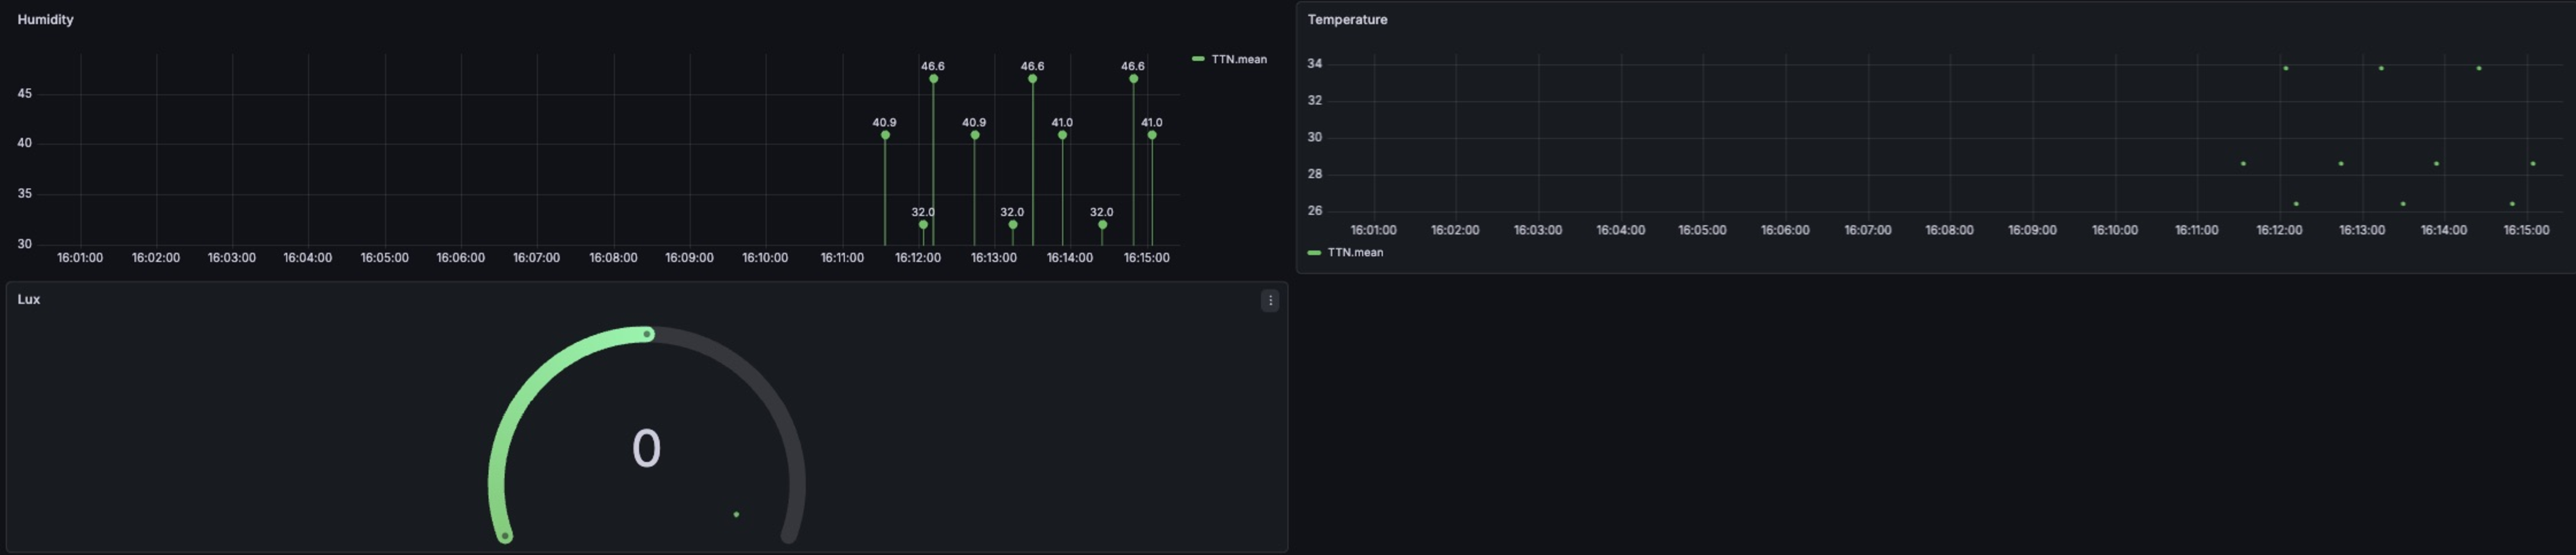
\includegraphics[width=0.8\linewidth]{Resources/Grafana.pdf} % <-- replace with your filename
    \caption{Grafana dashboard}
\end{figure}



\newpage
\section{Exercise 3 - MQTT Brokers}

For this exercise, I wrote a docker-compose file to run 2 MQTT brokers simultaneously in 2 different containers. In particular:
\begin{itemize}
    \item Each broker has its own container name;
    \item \texttt{broker\_a} is accessible at '\texttt{localhost:1883}';
    \item \texttt{broker\_a} is accessible at '\texttt{localhost:1884}'. 
\end{itemize}

\lstset{
    basicstyle=\ttfamily\small,
    backgroundcolor=\color{gray!10},
    frame=single,
    breaklines=true,
    keywordstyle=\color{blue},
}

\lstdefinelanguage{yaml}{
  morekeywords={true,false,null,y,n},
  sensitive=false,
  morecomment=[l]{\#},
  morestring=[b]",
  morestring=[b]',
}
% \newpage
\begin{lstlisting}[language=yaml]
services:
  broker_a:
    image: eclipse-mosquitto:latest
    container_name: broker_a
    ports:
      - "1883:1883"
    volumes:
      - ./mosquitto:/mosquitto
    networks:
      - sub-net

  broker_b:
    image: eclipse-mosquitto:latest
    container_name: broker_b
    ports:
      - "1884:1883"
    volumes:
      - ./mosquitto:/mosquitto
    networks:
      - sub-net

networks:
  sub-net:
    driver: bridge
\end{lstlisting}

You can find the docker-compose file showed above, visiting the following link: \url{https://github.com/lalb03/Assignments-AIoT-2025-26/tree/9867300dca86d1b2c51eddc934450566e5989297/MQTT}
\section{Exercise 4 and 5: Telegram Bot}

Following the guide, I developed a Telegram bot that uses the \textit{Open-Meteo API} to fetch the current weather in Padua. 

In particular, every time a user sends the command "\texttt{/getdata}", the Telegram bot makes an HTTP call to the \textit{Open-Meteo API}. Once it receives the response, it sends the data back to the user and stores the measurement in a local database.

All available commands are the following:
\begin{itemize}
    \item "\texttt{/start}": starts the conversation and shows the list of available commands;
    \item "\texttt{/getdata}": retrieves the current temperature in Padua;
    \item "\texttt{/history}": returns the last 10 measurements;
    \item "\texttt{/average}": returns the average temperature over all measurements stored in the database;
    \item "\texttt{/max}": returns the maximum temperature stored in the database;
    \item "\texttt{/min}": returns the minimum temperature stored in the database.
\end{itemize}

The code of the bot is available at the following link: \url{https://github.com/lalb03/Assignments-AIoT-2025-26/blob/b01b02599151ea6dd1423e50dac6728c923c3610/Telegram_bot/tel_ex-2.py}
\bigskip

In the following page, you can find a screenshot of a conversation with the bot.
\begin{figure}[h!]
    \centering
    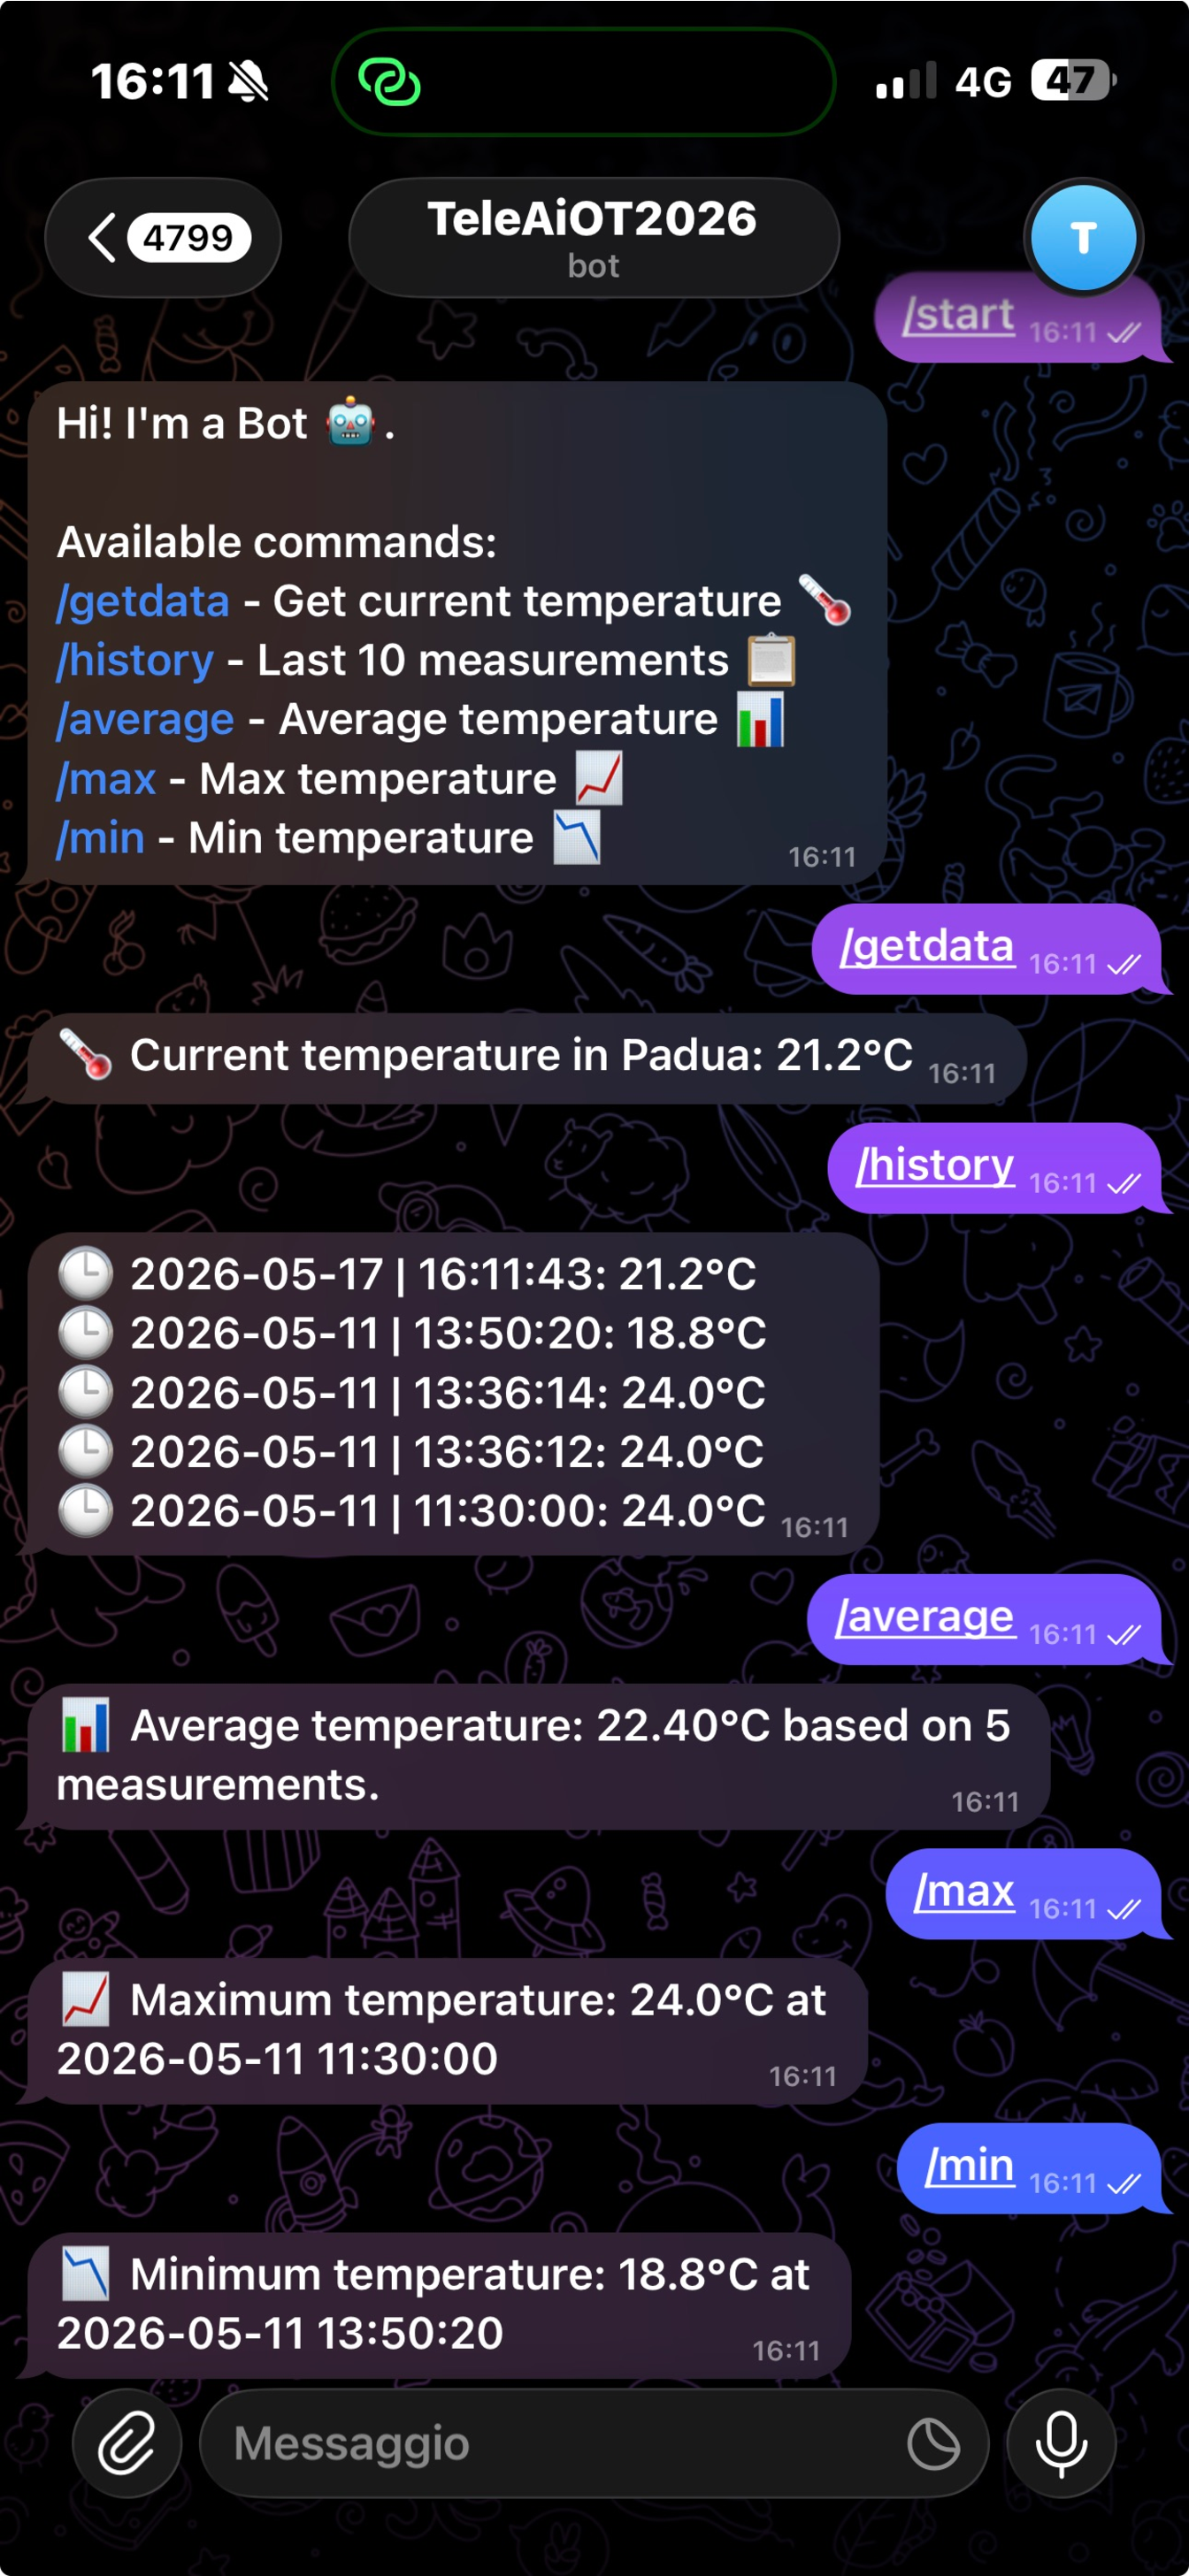
\includegraphics[width=0.5\linewidth]{Resources/Screenshot_chat.pdf}
    \caption{Screenshot of a conversation}
\end{figure}




\end{document}

